\chapter{Part 3}

\section{Introduction}
%• Very brief introduction of the overall problem setting (< page
%max)

Now describe the setup for the FlexRay modeling part, Figure \ref{fig:FRdia} shows the most important given parts and also the tree view in Inchron along with the FlexRay bus connections.

\begin{figure}[h!]
	\begin{center}
		
			\begin{tabular}{cc}
				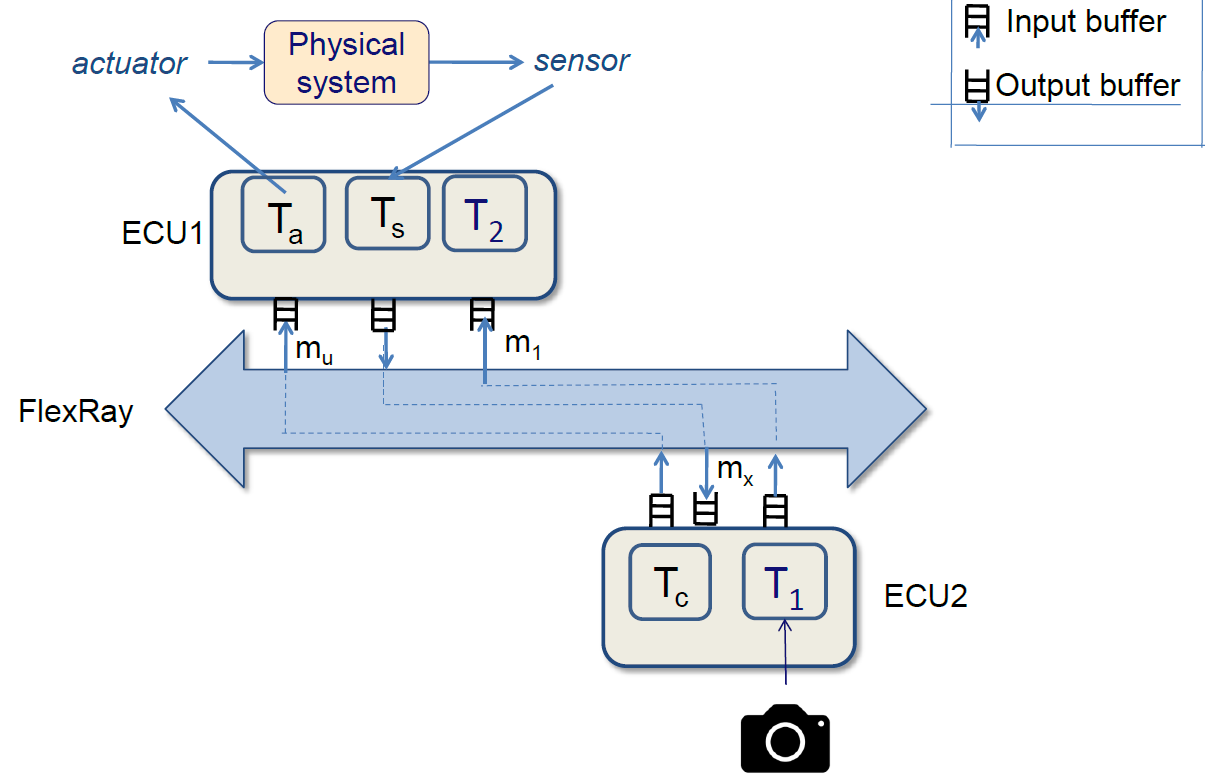
\includegraphics[width=0.5\linewidth]{img/FR-diagram} & 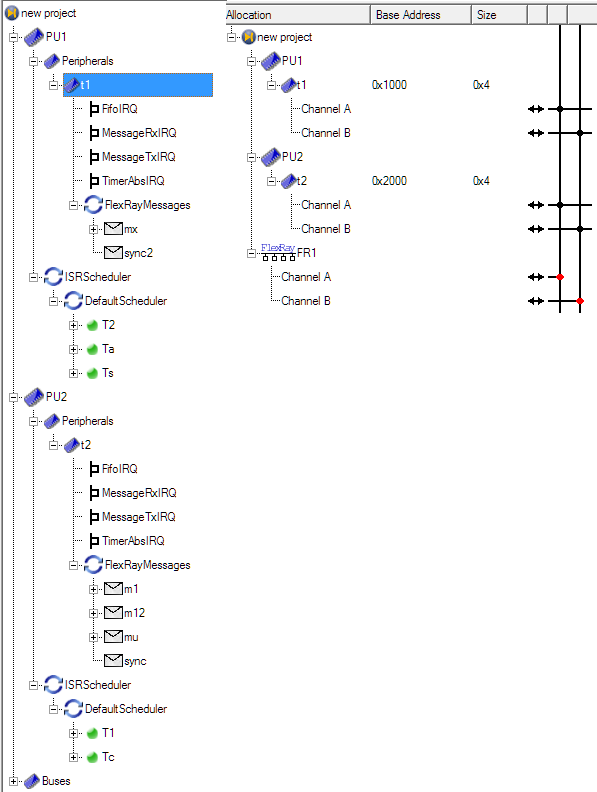
\includegraphics[width=0.35\linewidth]{img/FR-setup} \\
			\end{tabular}
			\caption{On the left, system diagram and on the right the tree view and architecture of the Inchron project. }
		\label{fig:FRdia}
	\end{center}
\end{figure}

The main purpose in this part is to firstly create a theoretical analysis to be able to model the FlexRay in Inchron. Then seeing how the implementation is doing in the model and optimize any timings that have room for change. 

\section{Answering the questions}


\begin{enumerate}
	\item \textit{What is the maximum cycle length possible? }
	
	The given cycle length is 4 ms so that is the maximum cycle length in our case.
	
	\item \textit{What are the maximum possible durations for:}
	
	\begin{enumerate}
			\item \textit{static slot?} If considering static slots then size of 0.5 ms should be the largest one (largest execution time considered of all messages AND tasks for easy scheduling) then maximum slot number is $\frac{4 \; ms}{0.5 \; ms} = 8$
			
			\item\textit{ dynamic slot? } This is not really relevant anymore were this part of Inchron did not work. But as example only dynamic considering a constant size of 0.25 ms: $\frac{4 \; ms}{0.25 \; ms} = 16 $ slots total
			
			\item \textit{Network idle time? }This will maintain synchronization between the two ECUs and for each it takes one slot so in total this is taking up two slots $= 2 \; slots \cdot 0.5 \; ms = 1 \; ms$.
	\end{enumerate}	
	
	\item\textit{ Derive the implicitly defined parameters (e.g., no. of minislots).}
	
	\item\textit{ Why do you need idle phase within a dynamic slot?} There is some idle time needed to react correctly on the coming messages to dynamic slots.
	
	\item \textit{Does the above parameters conform to FlexRay specification?} Not sure if this question still holds after the changes is assignment last minute after Inchron stopped working but the parameters for the FlexRay that we designed are working in Inchron. 
	
\end{enumerate}


\subsection{Theoretical analysis versus actual implementation}
%Comment on differences from the theoretical analysis and actual implementation
The theoretical analysis was done on paper with most parameters known and then model in Inchron to validate the behavior. There are obvious differences concerning cold start and such that will differ in actual implementation and in theory. But is is possible to counteract this be at least assuming a difference, not knowing how much they will vary.

\section{Design decision}
%• Your design decision and justification.
Firstly when starting design of theoretical analysis, it was done on paper to figure out the order of the messages and tasks within the static slots and which should go in the dynamic slot. The largest message would be best put in the dynamic slot, $m_1$. Then when realizing that the dynamic slots are not behaving correctly in Inchron, then it was decided to use only static slots. Then a problem arose, the size of each static slot is only 200 bytes but $m_1$ is 290 bytes. Thus splitting it up to two will do the trick.

It is very important to note that communication is included in the theoretical analysis but in Inchron they were skipped to lower the complexity but still there is room for everything and they are encountered for. In Figure \ref{fig:FRdrawing} the analysis on paper is showed for both ECUs and the FlexRay and how the messages are executing.
\begin{figure}[h!]
	\begin{center}
		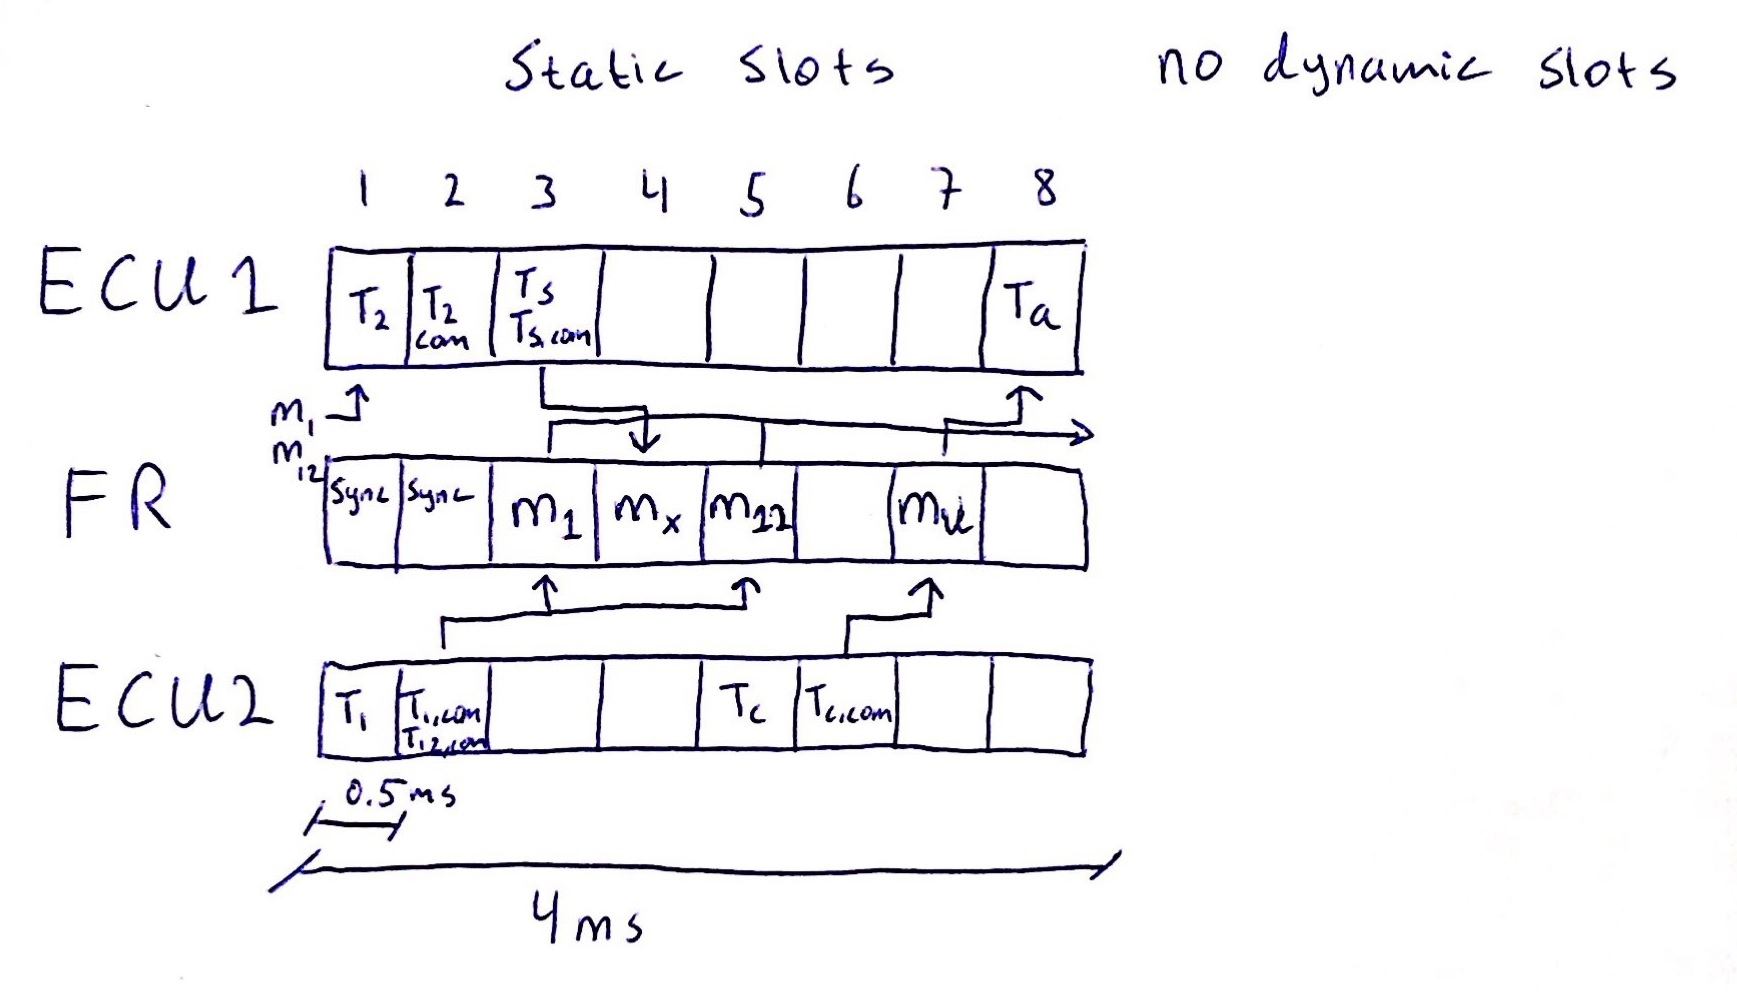
\includegraphics[width=0.9\linewidth]{img/FR-drawing-2}
		\caption{A sketch of the scheduling showing both ECUs and their connections to according sending or receiving messages}
		\label{fig:FRdrawing}
	\end{center}
\end{figure}

After applying this setup, exact parameters are shown in the results, to the model it showed that the tasks were staring before their cycle was actually happening. By measuring the exact offset it was possible to add it to all the tasks and messages to make the systems behave correctly. 

\begin{figure}[h!]
	\begin{center}
		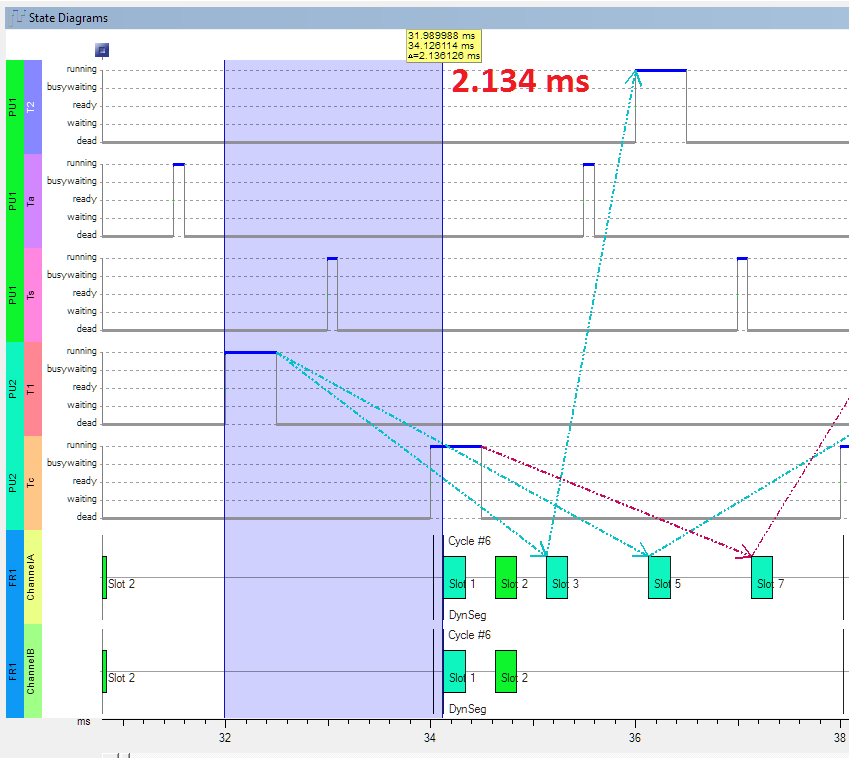
\includegraphics[width=0.8\linewidth]{img/FR-offset}
		\caption{Before optimization/offset the tasks are not hitting the start of the cycle, in fact all of the tasks are too early by 2.134 ms as seen in this figure.}
		\label{fig:FRoffset}
	\end{center}
\end{figure}



\section{Results}

The solution to the design problem can be seen in Table \ref{tab:flextsk} and \ref{tab:flexmsg} that shows the offset in the FlexRay for each of the messages and also the offsets for each of the tasks. 

For the tasks in Table \ref{tab:flextsk} the offsets tells from which millisecond the task will start in each cycle (according to Figure \ref{fig:FRdrawing}), period tells how frequently in milliseconds it will happen and execution is from the given information. 

Then for the messages the slot had the same purpose as the offset but is can be shown in the FlexRay slots 1-8 like shown in  Table \ref{tab:flexmsg} and then repetition wi shows 

\begin{table}[htbp!]
\centering
\begin{tabular}{|l|l|l|l|}
\hline
   & Offset(ms) & Period(ms) & ExecutionTime(ms) \\ \hline
   $ECU_2$ & & & \\ \hline
   $T_1$ & 0          & 8          & 0.5               \\ \hline
   $T_c$ & 2          & 4          & 0.5               \\ \hline
   $ECU_1$ & & & \\ \hline
	$T_2 $& 0          & 8          & 0.5               \\ \hline
	$T_s$ & 1          & 4          & 0.1               \\ \hline
	$T_a$ & 3.5        & 4          & 0.1               \\ \hline

\end{tabular}
\label{tab:flextsk}
\caption{Design of Tasks showing offsets, period and execution time}
\end{table}


\begin{table}[htbp!]
	\centering
	
	\begin{tabular}{|l|l|l|l|}
		\hline
		& Slot & Base & Repetition \\ \hline
		$m_1$  & 3    & 0    & 2          \\ \hline
		$m_{12}$ & 5    & 0    & 2          \\ \hline
		$m_x$  & 4    & 0    & 1          \\ \hline
		$m_u$  & 7    & 0    & 1          \\ \hline
	\end{tabular}
	\label{tab:flexmsg}
	\caption{Design of messages showing which slot in the FlexRay it starts, which cycle is the base and then how frequently}
\end{table}

Then it is important to show Figure \ref{fig:FRdiagram} which shows the end diagram of the system after adding mentioned inital offsets to the tasks.
\begin{figure}[h!]
	\begin{center}
		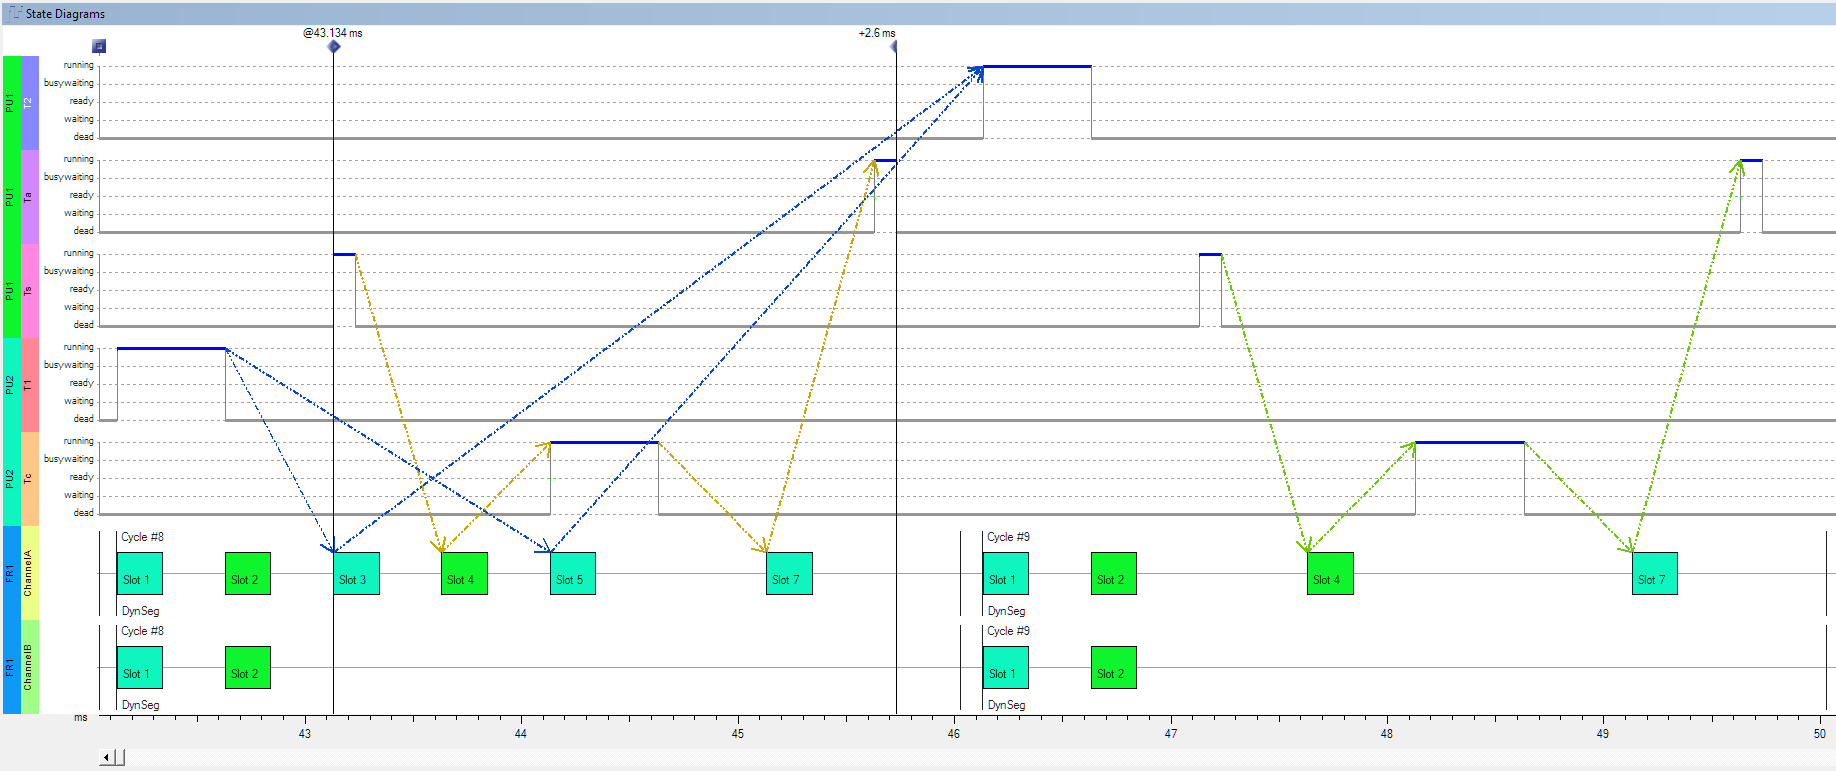
\includegraphics[width=0.9\linewidth]{img/FR-state-Diagram}
		\caption{The fully done and working version of the system where all tasks are in the right place receiving and sending messages like the theoretical analysis says it would}
		\label{fig:FRdiagram}
	\end{center}
\end{figure}

\section{Conclusions}

The final version of the parameters work as expected counteracting the initial offset. The reason for the initial offset is partially unknown but it is likely caused by the coldstart and obviously the synchronization is not behaving exactly as set to.